\graphicspath{{content/chapters/literature_review/other_compositional_models/figures}}

\section{Other Compositional Models}
\label{sec:other_compositional_models}

This section will explore \gls{nmn} models that come after the previously explored models but are still noteworthy due to improvements they make upon the original models.
Such models may either expand upon the neural module inventory with new module types or introduce structural changes to the model architecture.

\subsection{Meta Module Network}
\label{subsec:meta_module_network}

\gls{nmn} relies on its neural modules to understand and predict answers to \gls{vqa} questions.
However, as the complexity of the questions scales up, so would the module set need to be augmented accordingly which would lead to greater complexity.
This also means the model cannot be applied to new questions which use newly-seen tasks is introduced (such as training primarily for object relationships but then being tasked with counting and object-based arithmetic).
To address this, \citeauthor{chen_meta_2020} introduced \gls{mmn} \cite{chen_meta_2020} which uses general-purpose network modules instantiated on-the-fly according to the key-value pairs provided by the model.
Given a function recipe --- denoting what task types and parameters are required for an instance of a module --- a new module is instantiated according to this spec.
Using this approach, when an unseen recipe is encountered, a new module can still be instanced using pretrained parameters and similar trained recipes.
\todo[inline]{Expand on the structure and flow of the model, maybe mention Meta Learning which partly inspired the structure of the model \ldots}

\begin{figure}[htbp]
    \centering
    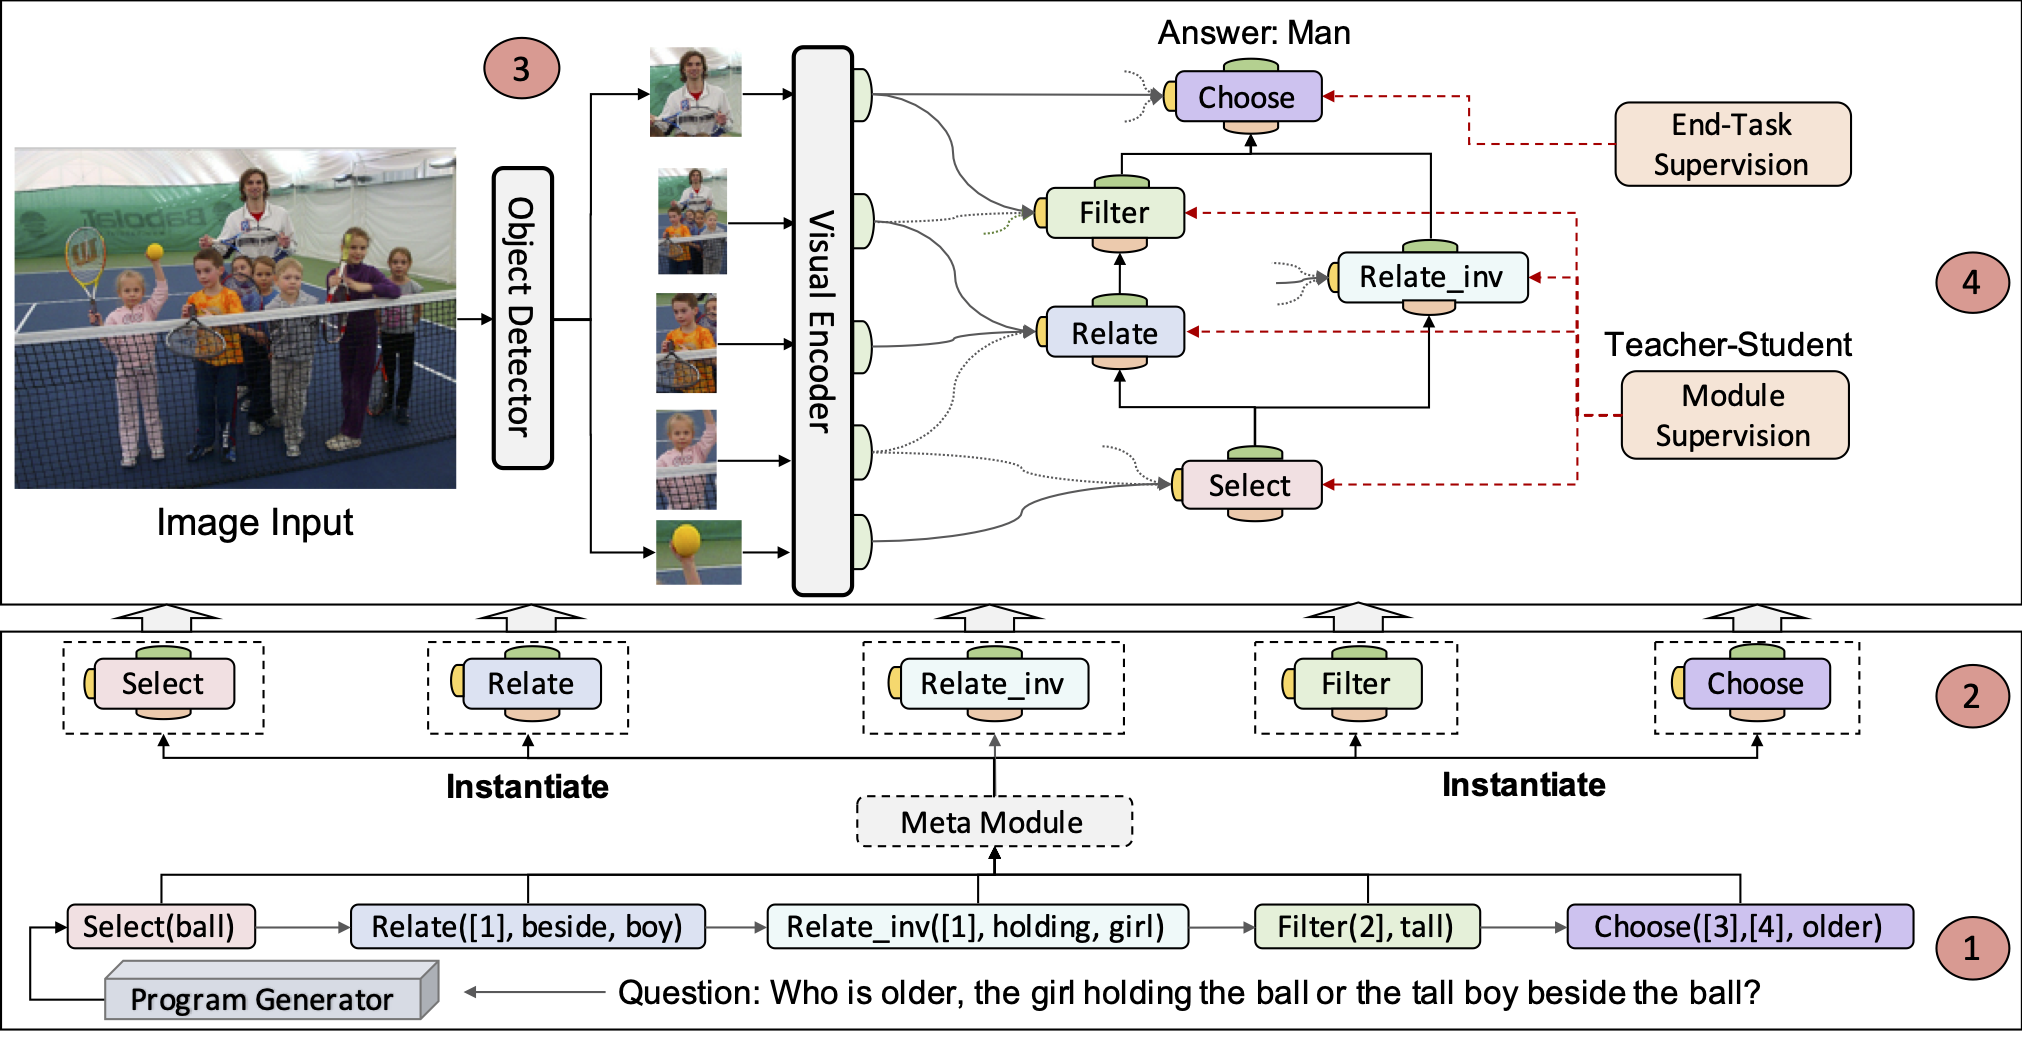
\includegraphics[width=.75\textwidth,keepaspectratio]{meta_module_network_overview}
    \captionsource(\acrshort{mmn} Overview){Architecture overview of the \acrshort{mmn} model, starting with the question-parsing (bottom) until it predicts the final answer (top) \label{fig:mmn_overview}}{\citeauthor{chen_meta_2020}\cite{chen_meta_2020}}
\end{figure}

\subsection{NMNs\pm}
\label{subsec:nmn_plus_minus}

\citeauthor{chen_teaching_2022} introduced NMNs\pm as an augmented \gls{nmn} which can basic arithmetic operations on questions.
The model supports addition and subtraction modules --- which take up to three number arguments --- and a date comparison function.
Using these additional modules, the model was able to outperform the original \gls{nmn} on an expanded text-only question-answer dataset known as DROP.
While the model is not trained on \gls{vqa} tasks, it would be safe to assume a similar performance improvement may be expected for those \gls{vqa} tasks that require arithmetic operations (such as comparing the counts of two object types in an image).

\todo[inline]{No module overview figure, maybe include a question-answer comparison between the models? (See Figure 1 in the published paper for information.)}

\subsection{Learnable Neural Module Network}
\label{subsec:learnable_neural_module_network}

Proposed by \citeauthor{pahuja_learning_2019} \cite{pahuja_learning_2019}, \gls{lnmn} is based on the \gls{snmn} model however, similar to the \gls{mmn} model, uses general-purpose neural modules instead of hard-coded ones.
The aim of this architecture was to explore the use of general-purpose neural modules as a robust and generalisable alternative to hard-coded modules and as such, does not achieve better outright performance compared to the \gls{snmn}.
Each neural module (or 'cell') is classified as either an Answer Module (outputs a memory features to be stored in the stack) or an Attention Module (outputs an attention map) and can either take 3 inputs or 4 inputs.
Each cell contains nodes which perform internal processing of cell inputs or prior node outputs and provide
To perform training on the model weights, the model performs gradient descent on a batch from the training set.
To perform training on the model cells and architecture, the model performs an alternative gradient descent step on a random sample batch from the validation set.
This approach to training both model cells and model weights is based on \gls{darts} which is an architecture search algorithm used for training \glspl{cnn} and \glspl{rnn_g}\cite{liu_darts_2019}.

